\chapter{Statistical Testing}\label{chap:stat_testing}
Inspired by \cite{hexeberg}, the performance of the proposed models will be compared on straight-line and curved trajectories independently. This comparison is intended to showcase the methods' ability to consistently predict reasonable trajectories and motivate further research into \acrshort{gp} based methods. However, the content of this chapter is not intended to showcase a perfect solution, and the methods are still heavily influenced by how the hyperparameters are selected, as well as any tuning parameters.

\section{Method}

The simulation will test the performance on a total of $700$ different test trajectories, where one half corresponds to straight-line trajectories and the remaining half consists of curved trajectories. Trajectories are selected from the dataset proposed in \cref{chap:ais}, and will have a total duration of between $15$ and $30$ minutes. The Direct GP and GP-EKF from \cref{chap:direct_gp} and \cref{chap:gp_ekf}, respectively, will be tested on the same scenarios as defined in \cref{chap:ais} and get access to the exact same training data.

Three different metrics -- trajectory error, path error and normalized estimation error squared -- will be used to compare the performance of the various methods.

\subsection{Trajectory Error}
The trajectory error is found by comparing the predicted mean position with the ground truth. As the predicted trajectory is simulated in discrete time, the points with the closest timestamps are used for comparison. The simulation will use $\Delta \tau = 10\text{ seconds}$, which yields a maximum error in time $\frac{\Delta \tau}{2} = 5 \text{ seconds}$, which is considered to be acceptable considering the time-horizon of between $15$ and $30$ minutes.
\subsection{Path Error}
The path error is defined as the closest point in the predicted trajectory to each point in the ground truth, under the constraint that the corresponding predicted timestamps must be monotonically increasing. In other words, the path cannot move backwards in time. Linear interpolation is used to get the path error at fixed timestamps to simplify the comparison.

\subsection{Normalized Estimation Error Squared}
For the uncertainty estimates to provide any value, the predictions must be consistent. In this context, the term consistency is borrowed from the term \textit{filter consistency} used when tuning Kalman filters \cite{sensorfusjon}. The idea is that prediction errors, on average, should scale with the state covariance. In other words, the model should not place much confidence in a prediction that is wrong while being highly confident when a prediction is correct. Consistency can also be interpreted using a frequentistic interpretation of probability, where after many predictions, the state uncertainty should reflect the actual error rate.

The \textit{\acrfull{nees}} is a metric that can be used to quantify consistency and is given by
\begin{equation}
    \text{NEES} = (\boldsymbol{x} - \hat{\boldsymbol{x}})^\intercal \boldsymbol{P}^{-1} (\boldsymbol{x} - \hat{\boldsymbol{x}})
\end{equation}

where $\boldsymbol{x}$ is ground truth and $\hat{\boldsymbol{x}}$ refers to the prediction.

Assuming that the prediction error follows a Gaussian distribution, the \acrshort{nees} follows a Chi-Squared distribution which can be used to form a confidence interval. Comparing the prediction errors with this confidence interval can then be used to get a sense of whether the estimated state uncertainty is consistent with the actual error rate.

\subsection{Comparing distributions - Boxplot}
The boxplot is used to visualize the distribution of the different metrics. The boxplot visualizes the estimated quartiles, i.e. the $25\%$, $50\%$, and $75\%$ quantiles, of the distribution. The "whiskers" show the range of values not considered to be outliers. Points outside of $[Q_{25} - 1.5 \text{ IQR}, Q_{75} + 1.5 \text{ IQR}]$ are considered outliers, where $\text{IQR} = Q_{75} - Q_{25}$ is the \text{inter-quartile range} \cite{matplotlib}.

\subsection{Interpolation}
The metrics will be compared at fixed $5$ minute intervals using linear interpolation. The error for short trajectories is not extrapolated, so there might be fewer available samples for the metrics when moving past $15$ minutes.

\subsection{Baseline - Constant Velocity Model}
As a basis of comparison, the \textit{\acrfull{cvm}} method is used as a baseline. The model uses the initial \acrshort{cog} and \acrshort{sog} to predict a straight line, where the vessel is assumed to keep a constant velocity and heading.

\subsection{Selecting test cases}
The two datasets from \cref{chap:ais} are used to perform the statistical testing.

However, $54\%$ of the dataset originates from only three ferries. Distinct discontinuities characterize the trajectories of these ferries as the vessels dock for short periods before moving back the same way they came. These discontinuities directly contradict the assumptions of smoothness made by the \acrshort{gp}s used in this thesis. Whether or not to include these vessels was a challenging decision, as a \acrshort{colav} will need to be able to handle ferries, just as any other vessel type. However, in a practical application, it is natural to distinguish between different vessel types and allow the use of more specialized models to handle cases such as frequently docking ferries. As no such distinction is made in this thesis, the statistical testing will be more insightful without using edge-cases for more than $50\%$ of the test cases. While it would be possible to not completely remove these vessels, i.e. perform subsampling, it is considered more confusing. Therefore, the samples from these three vessels are removed from the test set, though they are still present in the training set. This thesis has not proposed any method for filtering the training data based on the \acrshort{mmsi}; removing these vessels from the training set would be an unfair advantage.

The result is an artificial bias favoring the \acrshort{gp} framework proposed in this thesis, as the fraction of smooth trajectories has been artificially increased.

\subsubsection{Straigth-line trajectories}
The methods are first compared to the \acrshort{cvm} on simple straight-line trajectories. The statistics are based on $350$ randomly sampled trajectories without replacement that satisfy the following requirements:
\begin{enumerate}
    \item The sum of subsequent changes in \acrshort{cog} must be less than $30$ degrees, i.e. $\sum_i |(\mathcal{X}_{t+1} - \mathcal{X}_t)| \leq 30^\circ$. This requirement ensures a straight-line trajectory. Additional care is always taken to use the smallest possible difference as the angles $\mathcal{X} \in [0^\circ, 360^\circ)$ wraps around.
    \item There must be sufficient data available for training in the neighborhood around the initial starting point, with similar initial heading and speed. After sanitizing the dataset and removing irrelevant trajectories, at least $3$ trajectories need to be available for training.
    \item The overall duration of the trajectories must be between $15$ and $30$ minutes to be considered a test candidate.
\end{enumerate}

\subsubsection{Curved Trajectories}
The curved trajectory statistics are based on $350$ randomly sampled trajectories that satisfy the following requirements:
\begin{enumerate}
    \item The sum of subsequent changes in \acrshort{cog} must be greater than $40$ degrees, i.e. $\sum_i |(\mathcal{X}_{t+1} - \mathcal{X}_t)| \geq 40^\circ$. This requirement ensures a minimum curvature in the trajectory. Additional care is always taken to use the smallest possible difference as the angles $\mathcal{X} \in [0^\circ, 360^\circ)$ wraps around.
    \item There must be sufficient data available for training in the neighborhood around the initial starting point, with similar initial heading and speed. After sanitizing the dataset and removing irrelevant trajectories, at least $3$ trajectories need to be available for training.
    \item The overall duration of the trajectories must be between $15$ and $30$ minutes to be considered a test candidate.
\end{enumerate}

\subsection{Training Data}
The initial conditions for each test trajectory are considered a distinct scenario, and the relevant training data is selected according to the method proposed in \cref{chap:ais}. The requirements are restated here with the concrete values used for testing:

\begin{enumerate}
    \item The trajectories' initial position must be close to the target vessel's position $\boldsymbol{x}_0$. A fixed threshold at $||\Delta \boldsymbol{x}_0|| \leq 200 \text{ m}$ is used, where $\Delta \boldsymbol{x}_0$ is the difference between the target vessel's current position and the initial conditions of a potential training trajectory.
    \item The trajectories' initial \acrshort{cog} must be close to the target vessel's heading $\mathcal{X}$. A fixed threshold at $\mathcal{X} \pm 20^\circ$ is used, with additional care taken when the angles wrap.
    \item The trajectories' initial \acrshort{sog} must be close to the queried velocity $v$. A fixed threshold at $v \pm 4 \text{ knots}$ is used.
\end{enumerate}

Due to the way trajectories are generated from the \acrshort{ais} dataset, there will be significant overlaps between trajectories. Therefore, naively dividing the trajectories into a train and test set is considered insufficient, as sub-trajectories from the test set might also exist in the training set. Instead, the entire dataset is available for training, but all trajectories with identical MMSI and date as the test trajectory are removed before training. The date requirement ensures that trajectories for the same vessel can be used for training on any other day. There is still the possibility of leaking data from the test set if the trajectory moves past midnight, but this is assumed only to affect a negligible number of trajectories.


\section{Implementation}
The implementation details for each method are described in this section.

\subsection{Direct GP}
The excact \acrshort{gp} formulation is implemented using the \texttt{GaussianProcessRegressor} from the Python library, \textit{scikit-learn} \cite{scikit-learn}. The library supports all kernels introduced in \cref{chap:theory} and supports hyperparameter optimization using multiple restarts to avoid bad local optima.

The slightly more complicated kernel in \cref{eq:direct_gp_kernel} from \cref{chap:direct_gp} is used. This kernel is preferred over a single \acrshort{rbf} kernel as it simply yields the best performance across a range of different simulations. The noise term $\sigma^2$ is included as a White kernel and optimized like any other hyperparameter. The parameters are optimized for each test scenario, using $10$ random restarts to reduce the risk of bad local optima.

\subsection{GP-EKF}
The GP-EKF is tested with and without both the \acrshort{sl} and the \acrshort{pdaf} update steps, as well as using both finite difference and the \acrshort{cog}/\acrshort{sog} from the \acrshort{ais} dataset, resulting in $6$ different instances.

The GP-EKF requires more flexibility during development. Due to the need for calculating the gradient $\frac{\delta \vec{f}}{\delta \boldsymbol{x}}$, it is impractical to use existing \acrshort{gp} implementations. Due to the simple implementation of \cref{alg:gp_prediction}, it is easier to implement it from the ground up rather than adapting existing solutions.
The GP-EKF used in this thesis is therefore implemented directly in Python using only \textit{scipy}\cite{scipy} and \textit{numpy}\cite{numpy} to speed up linear algebra routines. The Cholesky decomposition in \cref{alg:gp_prediction} can be computed using \texttt{scipy.linalg.cho\_factor}, which calls a highly optimized LAPACK routine. Similarily, \texttt{scipy.linalg.solve\_\-trianglular} can be used to solve the lower triangular system of equations by forward substitution. The implementation of GP-EKF and the \acrshort{pdaf} update is then straightforward using \cref{alg:gp_ekf_prediction} and \cref{alg:gp_ekf_pdaf} from \cref{chap:gp_ekf}. The implementation used for the statistical testing use standardized training outputs $\boldsymbol{y}$.

For statistical testing, the proposed \acrshort{rbf} kernel from \cref{eq:dyngp_kernel} with independent length scales will be used due to its simplicity. More complicated kernels are avoided due to challenges with bad local optima during hyperparameter optimization.

The hyperparameters are tuned using the \acrshort{gp} implementation in the popular \textit{scikit-learn} \cite{scikit-learn} Python package. $10$ random restarts are used during optimization to reduce the risk of bad local minima. A lower bound constraint for the length scales is also used to avoid obvious overfitting and requires the length scales to be greater than $50$. Due to the wide variety of different scenarios on the training set, the hyperparameters are optimized for each iteration. This way, the robustness of the optimization is indirectly tested, as instances of bad local optima are included in the results.


The remaining parameters not found through \acrshort{ml} are tuned through trial and error on a few different trajectories.
The initial state uncertainty is set to $\boldsymbol{P}_0 = 500^2 \cdot \boldsymbol{I}$, which was found to work well during development. The \acrshort{pdaf} parameters are available in \cref{table:stats_pdaf_params} and the \acrshort{sl} parameters can be found in \cref{table:stats_sl_params}.

\begin{table}[h]
    \centering
    \begin{subtable}{0.49\textwidth}
        \begin{tabular}{|lll|}
            \textit{\textbf{Parameter}} &                                & \textit{\textbf{Value}}      \\ \hline
            Measurement noise           & $\boldsymbol{R}_{\text{PDAF}}$ & $500^2 \cdot \boldsymbol{I}$ \\
            Detection Probability       & $p_D$                          & $0.8$                        \\
            Clutter Rate                & $\lambda$                      & $2 \cdot 10^{-3}$            \\
            Gate Size                   & $g$                            & $2$
        \end{tabular}
        \caption{Parameters used for \acrshort{pdaf} update}
        \label{table:stats_pdaf_params}
    \end{subtable}
    \begin{subtable}{0.49 \textwidth}

        \centering
        \begin{tabular}{|lll|}
            \textit{\textbf{Parameter}} &                              & \textit{\textbf{Value}}      \\ \hline
            Noise                       & $\boldsymbol{R}_{\text{SL}}$ & $500^2 \cdot \boldsymbol{I}$ \\
            Search Radius               &                              & $50$                         \\
                                        &                              &                              \\
                                        &                              &
        \end{tabular}
        \caption{Parameters used for the SL update}
        \label{table:stats_sl_params}
    \end{subtable}
\end{table}



\section{Results}
The error metrics for straight-line and curved trajectories are available in \cref{table:stats_straight_line_error} and \cref{table:stats_curved_error} respectively, while the \acrshort{nees} results are available in \cref{table:stats_nees_straight} and \cref{table:stats_nees_curved}. All tables are found at the end of this chapter. Some hand-picked test scenarios are also included in \cref{chap:gp_ekf_examples} for the different GP-EKF variations.

This section will take a hierarchical approach, where the GP-EKF using finite-difference for training data is considered the basic configuration of the GP-EKF and will be used as a baseline when comparing the different variants of the GP-EKF. Unless explicitly stated otherwise, it is safe to assume that the GP-EKF uses finite-difference and no update step. For comparing specific combinations, the reader is referred to \cref{table:stats_straight_line_error} and \cref{table:stats_curved_error}.

As a base of comparison, the Direct GP and GP-EKF are compared to the \acrshort{cvm} on both straight-line and curved trajectories in \cref{fig:stats_both_vs_cvm}. On straight-line trajectories, both methods perform worse than the \acrshort{cvm} with higher trajectory error for all respective quartiles. As expected, the \acrshort{cvm} struggles on curved trajectories, whereas both the Direct GP and GP-EKF approaches perform significantly better with both lower median error and spread. The Direct GP approach performs slightly better than the GP-EKF, with lower median trajectory error and lower spread for both straight-line and curved trajectories. When comparing the path error for straight-line trajectories in \cref{table:stats_straight_path_err}, the GP-EKF performs consistently better than the Direct GP approach, with lower mean and median path error. The GP-EKF even outperforms the \acrshort{cvm} on straight-line paths when predicting beyond $15$ minutes.

Both the Direct GP and the GP-EKF approach perform better on curved trajectories as opposed to straight-line trajectories. After manually inspecting the test cases, it appears that many of the straight-line test cases belong to slow-moving vessels that are part of longer curved trajectories.  The training samples used to fit the \acrshort{gp}s in these cases often contain samples from faster-moving vessels, making the \acrshort{gp}s overshoot in their predictions. This hypothesis is corroborated by the path error in \cref{table:stats_straight_path_err}, as the GP-EKF outperforms the \acrshort{cvm} on long straight-line paths.

Neither the Direct GP nor the GP-EKF yield consistent uncertainty estimates as found by comparing the \acrshort{nees} to the theoretical $\mathcal{X}^2$ quartiles in \cref{fig:stats_straigth_nees_basic} and \cref{fig:stats_curved_nees_basic}. For both methods, the \acrshort{nees} is especially bad for straight-line trajectories with estimated quartiles exceeding the theoretical quartiles, which is likely linked to the increased error for the straight-line trajectories. The Direct GP approach performs better than the GP-EKF, with the $25\%$ and $50\%$ quartiles close to the theoretical values, while the basic GP-EKF remains overconfident for all quartiles. The upper quartile for both methods exceeds the theoretical value for the $\mathcal{X}^2$ distribution.

\subsection{GP-EKF: Finite Difference vs. COG/SOG from AIS}

\begin{figure}[h]
    \centering
    \makebox[\textwidth][c]{
        \begin{subfigure}{0.65\textwidth}
            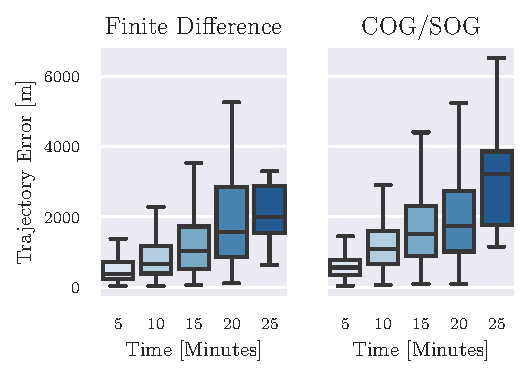
\includegraphics{figures/straight_line_stats/gp_cog_vs_fd.pdf}
            \caption{Straight-Line Trajectory}
        \end{subfigure}
        \begin{subfigure}{0.65\textwidth}
            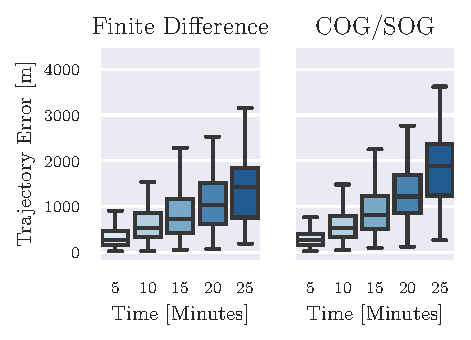
\includegraphics{figures/curved_line_stats/gp_cog_vs_fd.pdf}
            \caption{Curved Trajectory}
        \end{subfigure}
    }
    \caption{GP-EKF using finite differences and the \acrshort{cog} and \acrshort{sog} from the AIS dataset on $350$ trajectories. The finite differences approach performs consistently better, with lower median error and spread.}
    \label{fig:stats_gp_ekf_fd_vs_cog}
\end{figure}


A key design choice for the GP-EKF is deciding which data source to use for training. The model can either be trained using the \acrshort{cog} and \acrshort{sog} values contained in the \acrshort{ais} samples or by calculating numerical derivatives of the position through a finite-difference approach. \cref{fig:stats_gp_ekf_fd_vs_cog} compares the difference side-by-side. For straight-line trajectories, the results are remarkably similar. The finite difference approach seems to have a slight advantage on the lower quartile error at $\tau=25 \text{ minutes}$, though with an increased spread and the advantage is likely due to random errors. The finite difference performs slightly better than \acrshort{cog}/\acrshort{sog} for curved trajectories, especially as time increases, and has both lower median trajectory error and spread.

For the path errors in \cref{table:stats_straight_path_err} and \cref{table:stats_curved_path_err}, the results favor the \acrshort{cog}/\acrshort{sog} approach, with overall lower mean and median path errors when compared to the finite difference approach.

Using \acrshort{cog}/\acrshort{sog} yield a considerable \acrshort{nees} improvement over the finite difference approach, as seen in \cref{fig:stats_straigth_nees_cog_vs_fd} and \cref{fig:stats_curved_nees_cog_vs_df}. On curved trajectories, the estimated \acrshort{nees} quartiles is close to the theoretical values when using \acrshort{cog}/\acrshort{sog} as input data, while the finite difference approach yields overconfident results. A similar pattern is found for the median \acrshort{nees} values in \cref{table:stats_nees_straight} and \cref{table:stats_nees_straight} for all variants of the GP-EKF. 

\subsection{GP-EKF: Incorporating positions data}
The effect on the mean prediction for both the \acrshort{pdaf} and the \acrshort{sl} update procedures are compared to the basic GP-EKF configuration in \cref{fig:stats_gp_ekf_with_or_without_update}. The results are remarkably similar for both straight-line and curved trajectories. On closer inspection, there appears to be a slight advantage to using the \acrshort{pdaf} update step, but the improvement is within the margin of error, so it is not possible to draw any definitive conclusion.

However, the \acrshort{sl}, and, to some extent, the \acrshort{pdaf} update has a detrimental effect on the \acrshort{nees}, leading to even more overconfident predictions. This is apparent when comparing the GP-EKF NEES with and without the update steps in \cref{fig:stats_straight_nees_update} and \cref{fig:stats_curved_nees_update}, as the \acrshort{nees} for the \acrshort{sl} update explodes compared to the basic GP-EKF method. Similar patterns are found in \cref{table:stats_nees_straight} and \cref{table:stats_nees_curved} regardless of whether the GP-EKF is trained with finite difference or \acrshort{cog}/\acrshort{sog} data.

\begin{figure}
    \centering
    \begin{subfigure}{\textwidth}
        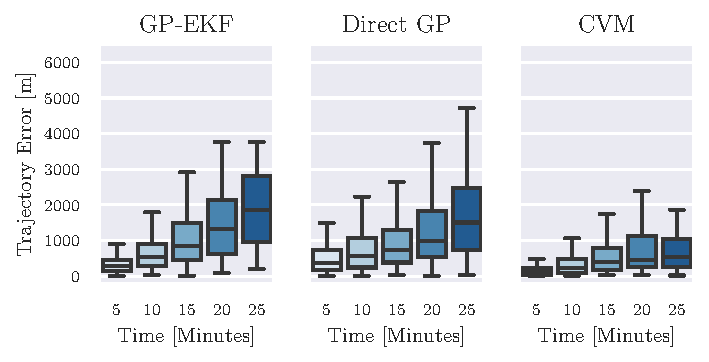
\includegraphics[width=\textwidth]{figures/straight_line_stats/both_vs_cvm.pdf}

        \caption{Straight-line trajectories.}
        \label{fig:stats_curved_both_vs_cvm}
    \end{subfigure}
    \begin{subfigure}{\textwidth}
        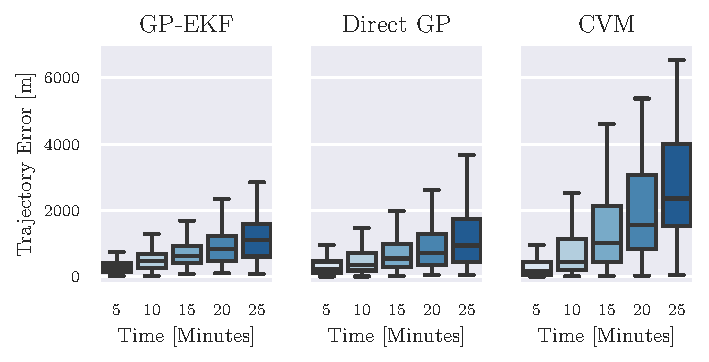
\includegraphics[width=\textwidth]{figures/curved_line_stats/both_vs_cvm.pdf}
        \caption{Curved trajectories.}
        \label{fig:stats_straight_both_vs_cvm}
    \end{subfigure}
    \caption{GP-EKF and Direct GP compared to a \acrshort{cvm} on $350$ straight-line and $350$ curved trajectories. For straight-line trajectories, the \acrshort{cvm} outperforms both the GP-EKF and the Direct GP, while the Direct GP yield slightly better performance than the GP-EKF. For curved trajectories, the \acrshort{cvm} struggles as expected. Both the GP-EKF and the Direct GP yields far better results with lower error and lower spread, while Direct GP has the lowest overall trajectory error quartiles. Interestingly, both GP-EKF and Direct GP performs better on curved trajectories than straight-line trajectories, with lower overall error and spread.}
    \label{fig:stats_both_vs_cvm}
\end{figure}



\begin{figure}[h]
    \centering
    \begin{subfigure}{1\textwidth}
        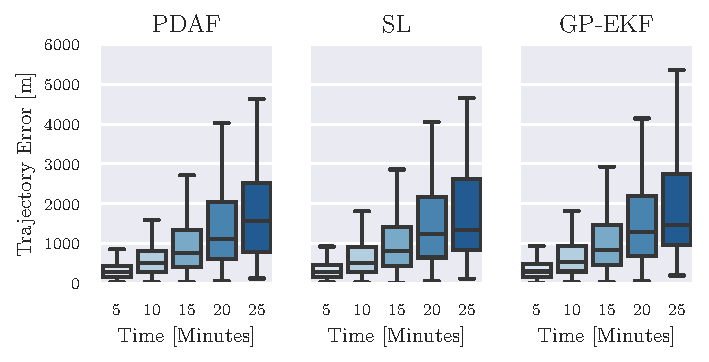
\includegraphics[width=\textwidth]{figures/straight_line_stats/gp_vs_update.pdf}
        \caption{Straight-Line Trajectories}
    \end{subfigure}
    \begin{subfigure}{1\textwidth}
        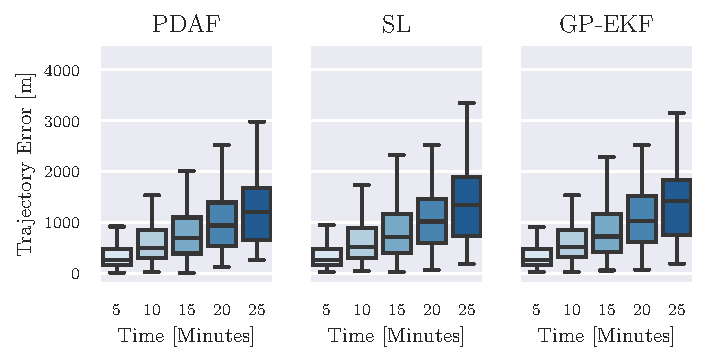
\includegraphics[width=\textwidth]{figures/curved_line_stats/gp_vs_update.pdf}
        \caption{Curved Trajectories}
    \end{subfigure}
    \caption{GP-EKF with and without the \acrshort{sl} and \acrshort{pdaf} updates on $350$ straight-line and $350$ curved trajectories. While there are some slight differences, the \acrshort{pdaf} and \acrshort{sl} update does not appear to have any considerable effect on the trajectory errors. On straight-line trajectories, the results are almost identicall across all three variants. On curved trajectories, the \acrshort{pdaf} yield slightly lower error for the median and upper quartiles, though the difference is well within the margin of error.}
    \label{fig:stats_gp_ekf_with_or_without_update}
\end{figure}

% \begin{figure}[h]
%     \centering
%     \begin{subfigure}{1\textwidth}
%         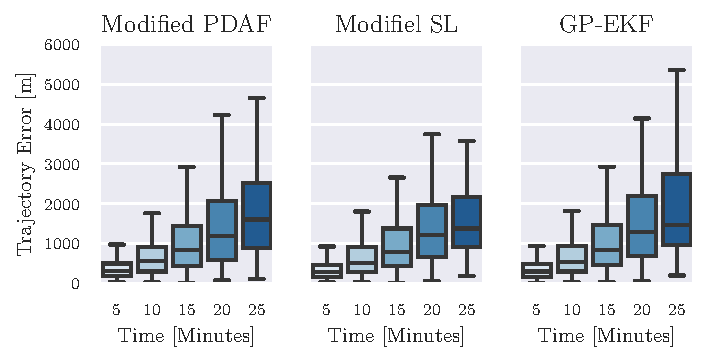
\includegraphics[width=\textwidth]{figures/straight_line_stats/gp_vs_update_no_P.pdf}
%         \caption{Straight-Line Trajectories}
%     \end{subfigure}
%     \begin{subfigure}{1\textwidth}
%         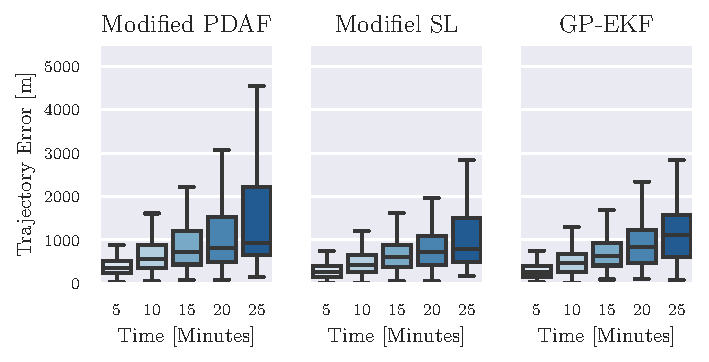
\includegraphics[width=\textwidth]{figures/curved_line_stats/gp_vs_update_no_P.pdf}
%         \caption{Curved Trajectories}
%     \end{subfigure}
%     \caption{GP-EKF with and without the modified \acrshort{sl} and \acrshort{pdaf} on curved trajectories for $350$ trajectories. The modified \acrshort{sl} performs better than the basic GP-EKF on straight-line trajectories for the upper $75\%$ quartile, while the modifed \acrshort{pdaf} performs about the same as the stock GP-EKF.  The modifed \acrshort{pdaf} performs worse than the basic GP-EKF on curved trajectories, while the modified \acrshort{sl} performs about the same.}
%     \label{fig:stats_gp_ekf_with_or_without_update_no_P}
% \end{figure}

\begin{figure}
    \centering
    \makebox[\textwidth][c]{
        \begin{subfigure}{0.6\textwidth}
            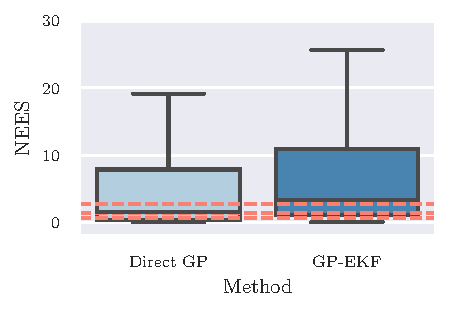
\includegraphics{figures/straight_line_stats/nees_vs_theoretical.pdf}
            \caption{Straight-Line Trajectory NEES Baseline}
            \label{fig:stats_straigth_nees_basic}
        \end{subfigure}
        \begin{subfigure}{0.6\textwidth}
            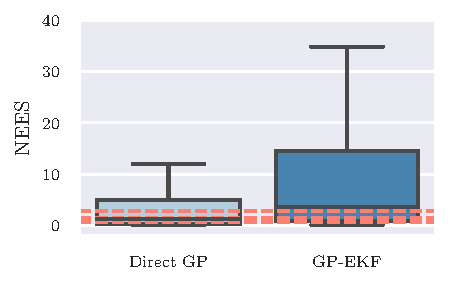
\includegraphics{figures/curved_line_stats/nees_vs_theoretical.pdf}
            \caption{Curved Trajectory NEES Baseline}
            \label{fig:stats_curved_nees_basic}
        \end{subfigure}
    }
    \makebox[\textwidth][c]{
        \begin{subfigure}{0.6\textwidth}
            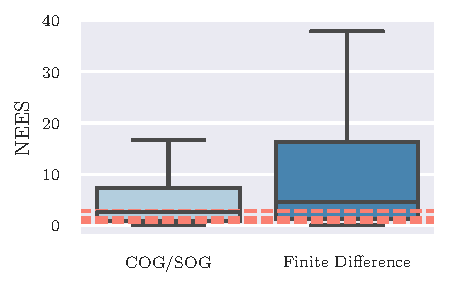
\includegraphics{figures/straight_line_stats/nees_vs_theoretical_cog_vs_fd.pdf}
            \caption{Straight-Line Trajectory COG/SOG vs Finite Difference}
            \label{fig:stats_straigth_nees_cog_vs_fd}
        \end{subfigure}
        \begin{subfigure}{0.6\textwidth}
            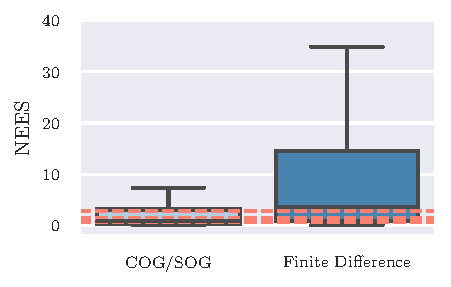
\includegraphics{figures/curved_line_stats/nees_vs_theoretical_cog_vs_fd.pdf}
            \caption{Curved Trajectory COG/SOG vs Finite Difference}
            \label{fig:stats_curved_nees_cog_vs_df}
        \end{subfigure}
    }
    \makebox[\textwidth][c]{
        \begin{subfigure}{0.6\textwidth}
            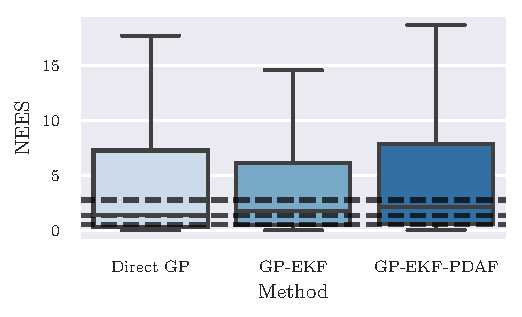
\includegraphics{figures/straight_line_stats/nees.pdf}
            \caption{Straight-Line Trajectory with update steps}
            \label{fig:stats_straight_nees_update}
        \end{subfigure}
        \begin{subfigure}{0.6\textwidth}
            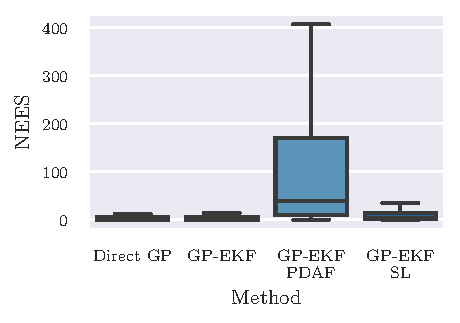
\includegraphics{figures/curved_line_stats/nees.pdf}
            \caption{Curved Trajectory with update steps}
            \label{fig:stats_curved_nees_update}
        \end{subfigure}
    }

    \caption{The NEES compared between the different methods. The top row compares the \acrshort{nees} for the Direct GP and the base GP-EKF to the theoretical quartile values for the $\mathcal{X}^2$ distribution (red dashed lines) and is intended as a base of comparison. The second row compares the difference in consistency between using \acrshort{cog}/\acrshort{sog} and finite difference as input data. The last row compares the effect of the update steps for the GP-EKF. The theoretical quartiles are not included in the last row due to the large differences in scale, and the reader is advised to use the Direct GP and basic GP-EKF for comparison.}

\end{figure}

% On straight-line trajectories, the $25\%$ and $50\%$ quartiles correspond well with the theoretical values for the $\mathcal{X}^2$ distribution for all methods. The \acrshort{pdaf} update step does, however, reduce the predicted uncertainty, leading to increased overconfidence. In addition, the estimated \acrshort{nees} distribution has a much fatter right-tail than the theoretical $\mathcal{X}^2$ distribution, leading to an estimated $75\%$ quartile far outside the theoretical values.

% On curved trajectories, the GP-EKF with and without PDAF is consistently overconfident. The theoretical quartiles are not plotted due to the large y-axis. The direct \acrshort{gp} approach performs significantly better, which is why a separate plot in \cref{fig:stats_curved_nees_direct} is added to compare it to theoretical quartiles.




\begin{table}[b]
    \begin{subtable}{\textwidth}
        \makebox[\textwidth][c]{
            \begin{tabular}{lllrrrrr}
                \toprule
                        &                & Time [Minutes]    & 5   & 10  & 15   & 20   & 25   \\
                Summary & Method         & Training Source   &     &     &      &      &      \\
                \midrule
                Mean    & CVM            & COG/SOG from AIS  & 172 & 383 & 623  & 786  & 772  \\
                        & Direct GP      & Position          & 603 & 720 & 944  & 1269 & 1727 \\
                        & GP-EKF         & COG/SOG from AIS  & 328 & 668 & 1090 & 1560 & 2048 \\
                        &                & Finite Difference & 331 & 656 & 1029 & 1417 & 1917 \\
                        & GP-EKF w/ PDAF & COG/SOG from AIS  & 331 & 668 & 1070 & 1494 & 1921 \\
                        &                & Finite Difference & 332 & 657 & 1025 & 1392 & 1856 \\
                        & GP-EKF w/ SL   & COG/SOG from AIS  & 325 & 654 & 1048 & 1489 & 1972 \\
                        &                & Finite Difference & 334 & 663 & 1025 & 1414 & 1891 \\
                \midrule
                Median  & CVM            & COG/SOG from AIS  & 94  & 226 & 387  & 463  & 549  \\
                        & Direct GP      & Position          & 367 & 562 & 727  & 978  & 1509 \\
                        & GP-EKF         & COG/SOG from AIS  & 295 & 575 & 883  & 1505 & 1911 \\
                        &                & Finite Difference & 298 & 537 & 851  & 1325 & 1868 \\
                        & GP-EKF w/ PDAF & COG/SOG from AIS  & 301 & 554 & 850  & 1401 & 1845 \\
                        &                & Finite Difference & 299 & 529 & 822  & 1250 & 1802 \\
                        & GP-EKF w/ SL   & COG/SOG from AIS  & 297 & 526 & 829  & 1324 & 1805 \\
                        &                & Finite Difference & 299 & 536 & 848  & 1315 & 1782 \\
                \bottomrule
            \end{tabular}

        }
        \caption{Trajectory errors in meters}
        \label{table:stats_straight_traj_err}
        \vspace*{0.5cm}
    \end{subtable}
    \begin{subtable}{\textwidth}
        \makebox[\textwidth][c]{
            \begin{tabular}{lllrrrrr}
                \toprule
                        &                & Time [Minutes]    & 5   & 10  & 15  & 20  & 25  \\
                Summary & Method         & Training Source   &     &     &     &     &     \\
                \midrule
                Mean    & CVM            & COG/SOG from AIS  & 58  & 180 & 351 & 491 & 504 \\
                        & Direct GP      & Position          & 362 & 318 & 428 & 575 & 794 \\
                        & GP-EKF         & COG/SOG from AIS  & 82  & 158 & 245 & 283 & 330 \\
                        &                & Finite Difference & 92  & 194 & 309 & 360 & 394 \\
                        & GP-EKF w/ PDAF & COG/SOG from AIS  & 81  & 157 & 248 & 295 & 319 \\
                        &                & Finite Difference & 91  & 192 & 309 & 367 & 393 \\
                        & GP-EKF w/ SL   & COG/SOG from AIS  & 87  & 169 & 253 & 298 & 329 \\
                        &                & Finite Difference & 99  & 211 & 330 & 396 & 398 \\
                \midrule
                Median  & CVM            & COG/SOG from AIS  & 29  & 82  & 187 & 301 & 418 \\
                        & Direct GP      & Position          & 97  & 138 & 224 & 311 & 390 \\
                        & GP-EKF         & COG/SOG from AIS  & 60  & 97  & 150 & 182 & 262 \\
                        &                & Finite Difference & 62  & 121 & 188 & 210 & 237 \\
                        & GP-EKF w/ PDAF & COG/SOG from AIS  & 57  & 97  & 145 & 181 & 196 \\
                        &                & Finite Difference & 62  & 117 & 190 & 217 & 237 \\
                        & GP-EKF w/ SL   & COG/SOG from AIS  & 62  & 101 & 149 & 189 & 247 \\
                        &                & Finite Difference & 66  & 124 & 188 & 213 & 217 \\
                \bottomrule
            \end{tabular}
        }
        \caption{Path error in meters}
        \label{table:stats_straight_path_err}
    \end{subtable}
    \caption{Error summary for $350$ straight-line trajectories. Mean and median summary statistics are calculated for the trajectory and path error at fixed timestamps. Linear interpolation is used between samples. Errors for short trajectories are not extrapolated, and therefore not included in the $20$ and $25$ minute bins.}
    \label{table:stats_straight_line_error}
\end{table}

\begin{table}[b]
    \begin{subtable}{\textwidth}
        \makebox[\textwidth][c]{
            \begin{tabular}{lllrrrrr}
                \toprule
                        &                & Time [Minutes]    & 5   & 10   & 15   & 20   & 25   \\
                Summary & Method         & Training Source   &     &      &      &      &      \\
                \midrule
                Mean    & CVM            & COG/SOG from AIS  & 483 & 1184 & 1936 & 2148 & 2684 \\
                        & Direct GP      & Position          & 329 & 507  & 717  & 898  & 1305 \\
                        & GP-EKF         & COG/SOG from AIS  & 355 & 691  & 1009 & 1363 & 1895 \\
                        &                & Finite Difference & 400 & 706  & 897  & 1159 & 1552 \\
                        & GP-EKF w/ PDAF & COG/SOG from AIS  & 349 & 663  & 925  & 1167 & 1392 \\
                        &                & Finite Difference & 398 & 688  & 863  & 1078 & 1417 \\
                        & GP-EKF w/ SL   & COG/SOG from AIS  & 351 & 672  & 950  & 1260 & 1751 \\
                        &                & Finite Difference & 401 & 703  & 885  & 1134 & 1540 \\
                \midrule
                Median  & CVM            & COG/SOG from AIS  & 153 & 478  & 990  & 1441 & 2334 \\
                        & Direct GP      & Position          & 192 & 342  & 524  & 652  & 806  \\
                        & GP-EKF         & COG/SOG from AIS  & 273 & 532  & 821  & 1218 & 1880 \\
                        &                & Finite Difference & 262 & 522  & 721  & 1024 & 1421 \\
                        & GP-EKF w/ PDAF & COG/SOG from AIS  & 262 & 501  & 724  & 961  & 1133 \\
                        &                & Finite Difference & 261 & 502  & 699  & 939  & 1207 \\
                        & GP-EKF w/ SL   & COG/SOG from AIS  & 264 & 500  & 732  & 1036 & 1616 \\
                        &                & Finite Difference & 256 & 524  & 706  & 1018 & 1333 \\
                \bottomrule
            \end{tabular}
        }
        \caption{Trajectory Error in meters}
        \label{table:stats_curved_traj_err}
        \vspace*{0.5cm}
    \end{subtable}
    \begin{subtable}{\textwidth}
        \makebox[\textwidth][c]{
            \begin{tabular}{lllrrrrr}
                \toprule
                        &                & Time [Minutes]    & 5   & 10  & 15   & 20   & 25   \\
                Summary & Method         & Training Source   &     &     &      &      &      \\
                \midrule
                Mean    & CVM            & COG/SOG from AIS  & 214 & 587 & 1066 & 1354 & 1748 \\
                        & Direct GP      & Position          & 162 & 222 & 347  & 484  & 765  \\
                        & GP-EKF         & COG/SOG from AIS  & 159 & 283 & 428  & 451  & 573  \\
                        &                & Finite Difference & 194 & 357 & 466  & 492  & 502  \\
                        & GP-EKF w/ PDAF & COG/SOG from AIS  & 153 & 269 & 393  & 424  & 415  \\
                        &                & Finite Difference & 190 & 343 & 450  & 482  & 525  \\
                        & GP-EKF w/ SL   & COG/SOG from AIS  & 160 & 285 & 414  & 435  & 512  \\
                        &                & Finite Difference & 194 & 357 & 469  & 501  & 542  \\
                \midrule
                Median  & CVM            & COG/SOG from AIS  & 61  & 290 & 729  & 998  & 1497 \\
                        & Direct GP      & Position          & 72  & 132 & 225  & 280  & 344  \\
                        & GP-EKF         & COG/SOG from AIS  & 107 & 184 & 287  & 262  & 313  \\
                        &                & Finite Difference & 115 & 221 & 337  & 354  & 331  \\
                        & GP-EKF w/ PDAF & COG/SOG from AIS  & 100 & 171 & 242  & 226  & 219  \\
                        &                & Finite Difference & 114 & 210 & 315  & 355  & 385  \\
                        & GP-EKF w/ SL   & COG/SOG from AIS  & 103 & 186 & 249  & 249  & 240  \\
                        &                & Finite Difference & 117 & 222 & 319  & 376  & 362  \\
                \bottomrule
            \end{tabular}
        }
        \caption{Path error in meters}
        \label{table:stats_curved_path_err}
    \end{subtable}
    \caption{Error summary for $350$ curved trajectories. Mean and median summary statistics are calculated for the trajectory and path error at fixed timestamps. Linear interpolation is used between samples. Errors for short trajectories are not extrapolated, and therefore not included in the $20$ and $25$ minute bins.}
    \label{table:stats_curved_error}
\end{table}

\begin{table}[b]
    \makebox[\textwidth][c]{
        \begin{tabular}{lllrrrrr}
            \toprule
                    &                & Time [Minutes]    & 5     & 10     & 15     & 20     & 25     \\
            Summary & Method         & Training Source   &       &        &        &        &        \\
            \midrule
            Mean    & Direct GP      & Position          & 3.88  & 11.79  & 21.07  & 34.11  & 42.03  \\
                    & GP-EKF         & COG/SOG from AIS  & 2.88  & 83.09  & 112.68 & 67.59  & 24.88  \\
                    &                & Finite Difference & 25.66 & 79.24  & 153.31 & 64.10  & 185.33 \\
                    & GP-EKF w/ PDAF & COG/SOG from AIS  & 2.99  & 94.05  & 126.13 & 22.34  & 33.41  \\
                    &                & Finite Difference & 28.90 & 89.65  & 156.13 & 66.86  & 137.51 \\
                    & GP-EKF w/ SL   & COG/SOG from AIS  & 97.91 & 530.52 & 582.50 & 231.68 & 191.07 \\
                    &                & Finite Difference & 31.76 & 102.66 & 214.88 & 274.35 & 530.58 \\
            \midrule
            Median  & Direct GP      & Position          & 0.66  & 1.18   & 2.09   & 3.23   & 6.05   \\
                    & GP-EKF         & COG/SOG from AIS  & 1.30  & 2.39   & 3.36   & 5.64   & 7.92   \\
                    &                & Finite Difference & 1.80  & 4.10   & 7.26   & 12.52  & 25.43  \\
                    & GP-EKF w/ PDAF & COG/SOG from AIS  & 1.42  & 2.85   & 4.81   & 9.62   & 13.24  \\
                    &                & Finite Difference & 1.99  & 4.79   & 8.90   & 18.12  & 34.17  \\
                    & GP-EKF w/ SL   & COG/SOG from AIS  & 2.79  & 9.13   & 22.42  & 49.73  & 104.53 \\
                    &                & Finite Difference & 2.96  & 10.16  & 27.99  & 73.56  & 139.15 \\
            \bottomrule
        \end{tabular}
    }
    \caption{\acrshort{nees} for $350$ straight-line trajectories at fixed timestamps. Linear interpolation is used between samples.}
    \label{table:stats_nees_straight}
    \vspace*{0.5cm}
\end{table}
\begin{table}
    \makebox[\textwidth][c]{
        \begin{tabular}{lllrrrrr}
            \toprule
                    &                & Time [Minutes]    & 5     & 10    & 15     & 20     & 25     \\
            Summary & Method         & Training Source   &       &       &        &        &        \\
            \midrule
            Mean    & Direct GP      & Position          & 2.74  & 6.05  & 10.62  & 14.79  & 323.69 \\
                    & GP-EKF         & COG/SOG from AIS  & 6.08  & 65.25 & 235.24 & 8.86   & 15.08  \\
                    &                & Finite Difference & 36.86 & 28.44 & 94.24  & 39.93  & 89.61  \\
                    & GP-EKF w/ PDAF & COG/SOG from AIS  & 6.32  & 65.66 & 234.01 & 13.75  & 22.44  \\
                    &                & Finite Difference & 36.94 & 29.88 & 59.10  & 52.79  & 70.95  \\
                    & GP-EKF w/ SL   & COG/SOG from AIS  & 10.21 & 72.72 & 258.65 & 92.60  & 171.51 \\
                    &                & Finite Difference & 45.92 & 59.75 & 114.19 & 158.79 & 249.64 \\
            \midrule
            Median  & Direct GP      & Position          & 0.29  & 0.85  & 2.13   & 3.49   & 3.91   \\
                    & GP-EKF         & COG/SOG from AIS  & 0.62  & 0.76  & 0.91   & 1.18   & 1.85   \\
                    &                & Finite Difference & 1.53  & 3.09  & 4.89   & 8.72   & 18.20  \\
                    & GP-EKF w/ PDAF & COG/SOG from AIS  & 0.80  & 1.27  & 2.16   & 4.46   & 3.35   \\
                    &                & Finite Difference & 1.67  & 4.07  & 8.13   & 13.30  & 22.23  \\
                    & GP-EKF w/ SL   & COG/SOG from AIS  & 1.66  & 6.53  & 15.23  & 40.30  & 77.91  \\
                    &                & Finite Difference & 2.38  & 9.56  & 19.29  & 44.08  & 116.12 \\
            \bottomrule
        \end{tabular}
    }
    \caption{\acrshort{nees} for $350$ curved trajectories at fixed timestamps. Linear interpolation is used between samples.}
    \label{table:stats_nees_curved}
\end{table}


